\DiaryEntry{Prime Numbers, 1}{2020-11-09}{Number Theory}

\begin{definition}
    A integer $p>1$ is called prime, if its only positive divisors are $1$ and $p$. An integer greater than $1$ that is not prime is called a composite.
\end{definition}

Among the numbers below $10$, the primes are $2, 3, 5, 7$. The main interest in primes is that every composite number can be uniquely factored into primes.  For this result to prove, we need Euclid's Lemma.

\begin{theorem}
    If $p$ is a prime and $p \mid ab$, then $p \mid a$ or $p \mid b$.
\end{theorem}

We will use Bezout's identity which states that for integers $a, b$ with $\gcd(a,b) = d$, there exist integers $r,s$ such that

\bee
ar + bs = d \qed
\eee

If $p \mid a$, then we are done. So assume that $p \nmid a$. Since the only divisors of $p$ are $1$ and $p$, we have $\gcd(p,a) = 1$. Bezout's identity yields

\bee
p r + a s = 1 \rightarrow prb + sab = b
\eee

where we have multiplied both sides with $b$. Since $p \mid p$ and $p \mid ab$, $p$ divides the LHS and therefore also $p \mid b$. \qed

This can be extended to more than two factors; i.e. if

\bee
p \mid a_1 a_2 \cdots a_n
\eee

then

\bee
p \mid a_k, \text{ for some } 1 \leq k \leq n
\eee

We also have the following theorem.

\begin{theorem}\label{th:primes_01_01}
    If $p, q_1, q_2, \cdots q_k$ are all primes and $p | q_1 q_2 \cdots q_k$, then $p = q_k$ for some $k$, with $1 \leq k \leq n$.
\end{theorem}

From the previous theorem, we know that $p | q_k$ for some $k$ with $1 \leq k \leq n$. Being a prime, $q_k$ is not divisible by any positive integer other than $1$ or $q_k$ itself. Since $p>1$ (a prime has to be larger than $1$), we have to conclude $p = q_k$. \qed

\subsection{Fundamental Theorem of Arithmetic}

With all this in place, we can state the Fundamental Theorem of Arithmetic.

\begin{theorem}
    Every positive integer $n > 1$ is either a prime or a product of primes. This representation is unique, apart from the order in which the factors occur.
\end{theorem}

Proof: Either $n$ is prime (then we are done) or composite. In the latter case, there exists an integer $d$ satisfying $d \mid n$ and $1 < d < n$. Among all those integers, choose $p_1$ to be the smallest. THen $p_1$ must be a prime number; otherwise it too would have a divisor $q$ with $1 < q < p_1$: but then $q \mid p_1$ and $p_1 \mid n$ imply that $q \mid n$ and this contradicts the assumption that $p_1$ is the \emph{smallest} divisor of $n$.

We therefore can write $n = p_1 n_1$; $p_1$ is prime and $1 < n_1 < n$. Now we can continue the procedure from above: If $n_1$ is prime, we have found the required presentation $n = p_1 n_1$; otherwise we continue by factoring $n_1$. This proces has to come to an end (namely the $n_k$ are getting smaller and smaller) and we eventually arrive at the factorization

\bee
n = p_1 p_2 \cdots p_k
\eee

The uniqueness part of the theorem can be shown by contradiction: Assume

\bee
n = p_1 p_2 \cdots p_r = q_1 q_2 \cdots q_s, \quad r \leq s
\eee

where the $p_i$ and $q_i$ are all primes written in increasing order ($p_1 \leq p_2 \leq p_3 \cdots \leq p_r$ and analoguous for the $q_k$). This means we both allow for different factors and also a different number of the different factors.

Theorem \ref{th:primes_01_01} tells us that $p_1 = q_k$ for some $k$ and therefore $p_1 \geq q_1$. Similar reasoning gives $q_1 \geq p_1$ and therefore $p_1 = q_1$. We may cancel this common factor in above expression and arrive at

\bee
n = p_2 \cdots p_r = q_2 \cdots q_s
\eee

We could continue in this fashion and by the inequality $r \leq s$ we would then have

\bee
1 = q_{r+1}q_{r+2} \cdots q_s
\eee

which cannot be true because the $q_i$ are integers and must be larger than $1$. Therefore $r = s$ and we conclude that $p_k = q_k$ for all $k$. \qed

As a corollary we observe that this provides a canonical representation of a positive integer $n$,

\bee
n = p_1^{k_1} p_2^{k_2} \cdots p_r^{k_r}
\eee

where the $k_i$ are positive integers and the $p_i$ are primes with $p_1 < p_2 < \cdots < p_r$.

As an example, we have

\bee
804 = 2^2 \cdot 3 \cdot 67, \text{ and } \quad 5360 = 2^4 \cdot 5 \cdot 67
\eee

We can use this representation to calculate the gcd as follows. If

\bee
a = p_1^{k_1} p_2^{k_2} \cdots p_n^{k_n} , \text{ and } b = p_1^{j_1} p_2^{j_2} \cdots p_n^{j_n}
\eee

then

\bee
\gcd(a,b) = p_1^{\min(k_1, j_1)} p_2^{\min(k_2, j_2)} \cdots p_n^{\min(k_n, j_n)}
\eee

In our numeric example, we therefore have $\gcd(804, 5360) = 2^2 \cdot 67 = 268$.

\subsection{Number of Primes}

Leaving aside how the primality of a given integer can be determined (and if it is composite, how its prime factors can be determined), we may wonder how many primes there. This is answered by the following theorem.

\begin{theorem}
    There is an infinite number of primes.
\end{theorem}

We show this by contradiction: Assume there is a finite set of primes, $\Sc = \{p_1, p_2, \ldots, p_n\}$. We define $n = p_1 p_2 \cdot p_n$ which is divisible by all primes of $\Sc$. Now we consider

\bee
n+1 = p_1 p_2 \cdot p_n + 1
\eee

By the Fundamental Theorem we know that $n+1$ is either composite or a prime. If it were composite, none of the primes in $\Sc$ divides it, so $\Sc$ cannot contain \emph{all} primes. If $n+1$ were prime, it is also not contained in $\Sc$. In both cases, we conclude that $\Sc$ does not include all primes. \qed

We can illustrate the reasoning by means of an example. Consider the set of primes $\Sc_1 = \{2,3,5\}$, with $n = 30$ and $n+1 = 31$ which is prime. So $\Sc_1$ does not contain all primes. If we choose a larger set $\Sc_2 = \{2,3,5,7,11,13\}$ we have $n = 30030$, $n+1 = 30031 = 59 \cdot 509$ which is composite; however neither prime factor is contained in $\Sc_2$.

\subsection{Sieve of Eratosthenes}

The next question that arises is how to obtain prime numbers and / or factor composites. We first note that we can bound the prime factors of a composite number as follows: Let a composite $a = bc$ where $1 < b < a$ and $1 < c < a$. Without loss of generality we can assume $b \leq c$ and get $b^2 \leq bc = a$ from which we conclude $b \leq \sqrt{a}$. Since $b > 1$, it contains at least one prime factor $p$ and therefore $p \leq b \leq \sqrt{a}$. This result simplifies the factorization process as we need to check primes only up to $\sqrt{a}$ if they divide $a$.

As an example consider the integer $a = 2093$. We know that we need to check primes only up to $\sqrt{2093} \approx 45.7$; i.e. $46$. These are $2, 3, 5, 7, 11, 13, 17, 19, 23, 29, 31, 37, 41, 43$. The first prime to divide $2093$ is $7$ as $2093 = 7 \cdot 299$. Now we continue with $299$ which can have primes up to $\sqrt{299} \approx 17.2$; i.e. $18$. The first prime to divide $299$ is $13$, $299 / 13 = 23$. This is a prime and we are done; collecting factors we have

\bee
2093 = 7 \cdot 13 \cdot 23
\eee

The Sieve of Eratosthenes is a classical method to find primes below a certain threshold $N$. The scheme starts from a list of all integers below $N$ and then subsequently eliminating all composites by striking out all multiples $2p, 3p, 4p, \ldots$ of the primes $p \leq \sqrt{N}$. The integers left on the list are then primes.

As an example, consider a sieve for $N = 100$. We bootstrap the scheme with the smallest prime $2$ and strike out all multiples of $2$ in the list. The next "unstrucken" integer on the list is $3$ and we continue by striking all multiples of $3$ on the list. The integer $4$ has already been removed (as multiple of $2$), so we continue with $5$. Afterwards, we continue with $7$ and then there are no "unstrucken" integers up to $10 \leq \sqrt{N} = \sqrt{100}$; we are done.

The result is shown in the following Figure; multiples of $2$ are shown by $\backslash$, multiples of $3$ are shown by $/$, multiples of $5$ are shown by $-$, and multiples of $7$ are shown by a tilde.

\begin{figure}[H]
    \centering
    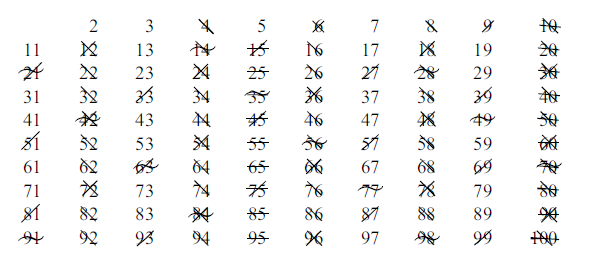
\includegraphics[scale=0.75]{images/primes_01_01.png}
\end{figure}


A simple Julia implementation looks as follows.

\begin{verbatim}
function sieve(N :: Int)
  is_primes = trues(N)
  is_primes[1] = false
  for i = 1:N
    if(is_primes[i] == true)
      j = 2*i
      if j > N
        return findall(is_primes)
      else
        is_primes[j:i:N] .= false
      end
    end
  end
end
\end{verbatim}


\subsection{Further Topics}

For a prime $p$, let us define $p^\#$ as the product of all primes below $p$. NUmbers of the form $p^\# + 1$ are called Euclidean integers. The first five integers, $2^\# + 1= 2 + 1 = 3, 3^\# = 2 \dot 3 + 1 = 6, \ldots 11^\# +1 = 2 \cdot 3 \cdot 5 \cdot 7 \cdot 11 +1 = 2311$ are all prime. The next ones, however, are not prime. An open question is whether there are infinitely many primes $p$ for which $p^\# + 1$ is prime. The largest known one is $392113^\# + 1$ and has approx. $170.000$ digits.

In the following, let $p_n$ denote the $n-$th prime in their natural ordering (e.g. $p_5 = 11$). We can bound primes using the proof of the infinite number of primes as

\bee
p_{n+1} \leq p_1 p_2 \cdots p_n + 1
\eee

This is based on the observation (see also above) that the RHS is not divisble by the primes $p_1, \ldots p_n$ and the RHS is either composite (in which case $p_{n+1}$ divides the RHS and must therefore be smaller) or a prime (in which case $p_{n+1}$ equals the RHS). \qed

Considering $p_5 = 11$, we have $p_5 \leq 2 3 5 7 + 1 = 211$ which is rather loose. There is a slightly tighter bound (shown without proof)

\bee
p_{n+1} \leq p_1 p_2 \cdots p_n - 1. 
\eee

Bonse's inequality provides a tighter bound, 

\bee
p_n^2  < p_1 p_2 \cdots p_{n-1}-1, \quad n \geq 5
\eee

For example, it yields $p_5^2 < 210, p_5 \leq 14$. A similar bound is given by

\bee
p_{2n} \leq p_2 p_3 \cdots p_n -2 \quad n \geq 3
\eee

which yields

\bee
p_5 < p_6 < 3 \cdot 5 - 2 = 13 \qed
\eee

There are also bounds for $p_n$ as function of $n$.

\begin{theorem}
    If $p_n$ is the $n-$th prime number, then $p_n \leq 2^{2^{n-1}}$.
\end{theorem}

We prove this using induction. Starting with $n=1$, we have $p_1 = 2 \leq 2^{2^{1}} = 4$ which is true. The induction step from $n \rightarrow n+1$ is as follows: We have

\begin{align*}
p_{n+1} & \leq p_1 p_2 \cdots p_n + 1 \\
        & \leq 2 2^2 2^4 \cdots 2^{2^{n-1}} + 1 = 2^{1 + 2 + 2^2 + 2^3 + \cdots 2^{n-1}} + 1 \\ 
        & \leq 2^{2^{n}-1} + 1
\end{align*}

where in the last inequality we have used the sum of the geometric series. We can "bound" $1$ by $1 \leq 2^{2^{n} - 1}$ for all $n$ and therefore have

\bee
p_{n+1} \leq 2^{2^{n}-1} + 2^{2^{n} - 1} = 2^{2^{n}} \qed
\eee

As a corollary, we note that

\begin{theorem}
    For $n \geq 1$, there are at least $n+1$ primes less than $2^{2^{n}}$.
\end{theorem}

From the previous theorem, we see that all $p_1, \ldots p_n$ are less than $2^{2^{n}}$. \qed

Bertrand's theorem (given without proof) states that between $n$ and $2n-2$ there is at least one prime. Using this, we can state the following theorem.

\begin{theorem}
    There exists a prime $p$ for which $p_n < 2^n, n \geq 2$ and $p_{n+1} < 2 p_n, n \geq 2$.
\end{theorem}

We use induction: For $n = 2, p_2 = 3 < 2^2 = 4$. Assume the theorem holds for $n$, we have $p_n < 2^n$. From Bertrand's conjecture it follows, that there is another prime $p$ for which $2^n \leq p \leq 2^{n+1}$; that is $p_n < p$. We therefore conclude that $p_{n+1} \leq p \leq 2^{n+1}$ which concludes the proof. \qed

Using our running example of $p_5 = 11$, we have $p_6 = 13 \leq 2 p_5 = 22$.

We finally consider \emph{repunits} which are integers consisting of $n$ ones; e.g. $R_2 = 11, R_5 =11111$. The general form is therefore

\bee
R_n = \frac{10^n - 1}{9}
\eee

These numbers are "special" as only very few of them are primes. The first primes are $n = 2, 19, 23, 317 \ldots$. For $n \leq 49000$, only nine repunits are prime and its is not known whether primes for larger $n$ exist.


%%% Local Variables:
%%% mode: latex
%%% TeX-master: "journal"
%%% End:
